\newpage
\section{Design}  
Here I will detail the design and implementation choices made for
\emph{AbTLinux}. Some early thoughts are Object Orientation and Ruby 
as implementation language. 

\subsection{Package structure}
A single package will have one file containing the entire structure needed for
installing the software it offers. This structure will be split into sections,
such as the following:
\begin{itemize}
  \item details\{\}
  \item pre\{\}
  \item configure\{\}
  \item pre-build\{\}
  \item build\{\}
  \item pre-install\{\}
  \item install\{\}
  \item post\{\}
\end{itemize}

This is rather flexible and open for debate, an example should be put together
for a rather complex package just to give an idea of what it will look like.
I think each section should be enclosed in curly brackets.

\subsubsection{Install locations}
Base system for AbTLinux will be in /usr, all others will be installed into /usr/local/*.
This will facilitate ease of usage within other Linux systems that follow the LSB/FHS.

\subsection{Configuration update tools}
Here I mean tools dealing with how we want configuration file updates to be
handled. Almost everything located in /etc of the Linux filesystem is considered
holy to a running system. They need to be updated sometimes when a new package
version is installed, but should never destroy an existing configuration. We
want to provide for the following:

\begin{itemize}
  \item view existing configuration file
  \item view new (default to install) configuration file
  \item allow editing to take place in old or new config file
  \item show user diff
  \item let user select one of the above options to install
\end{itemize}


\subsection{Package manager}
The AbT API outline can be found online at the AbTLinux website. The basic outline can be seen in Figure \ref{fig:abtapi}.

\begin{figure}
	\centering
	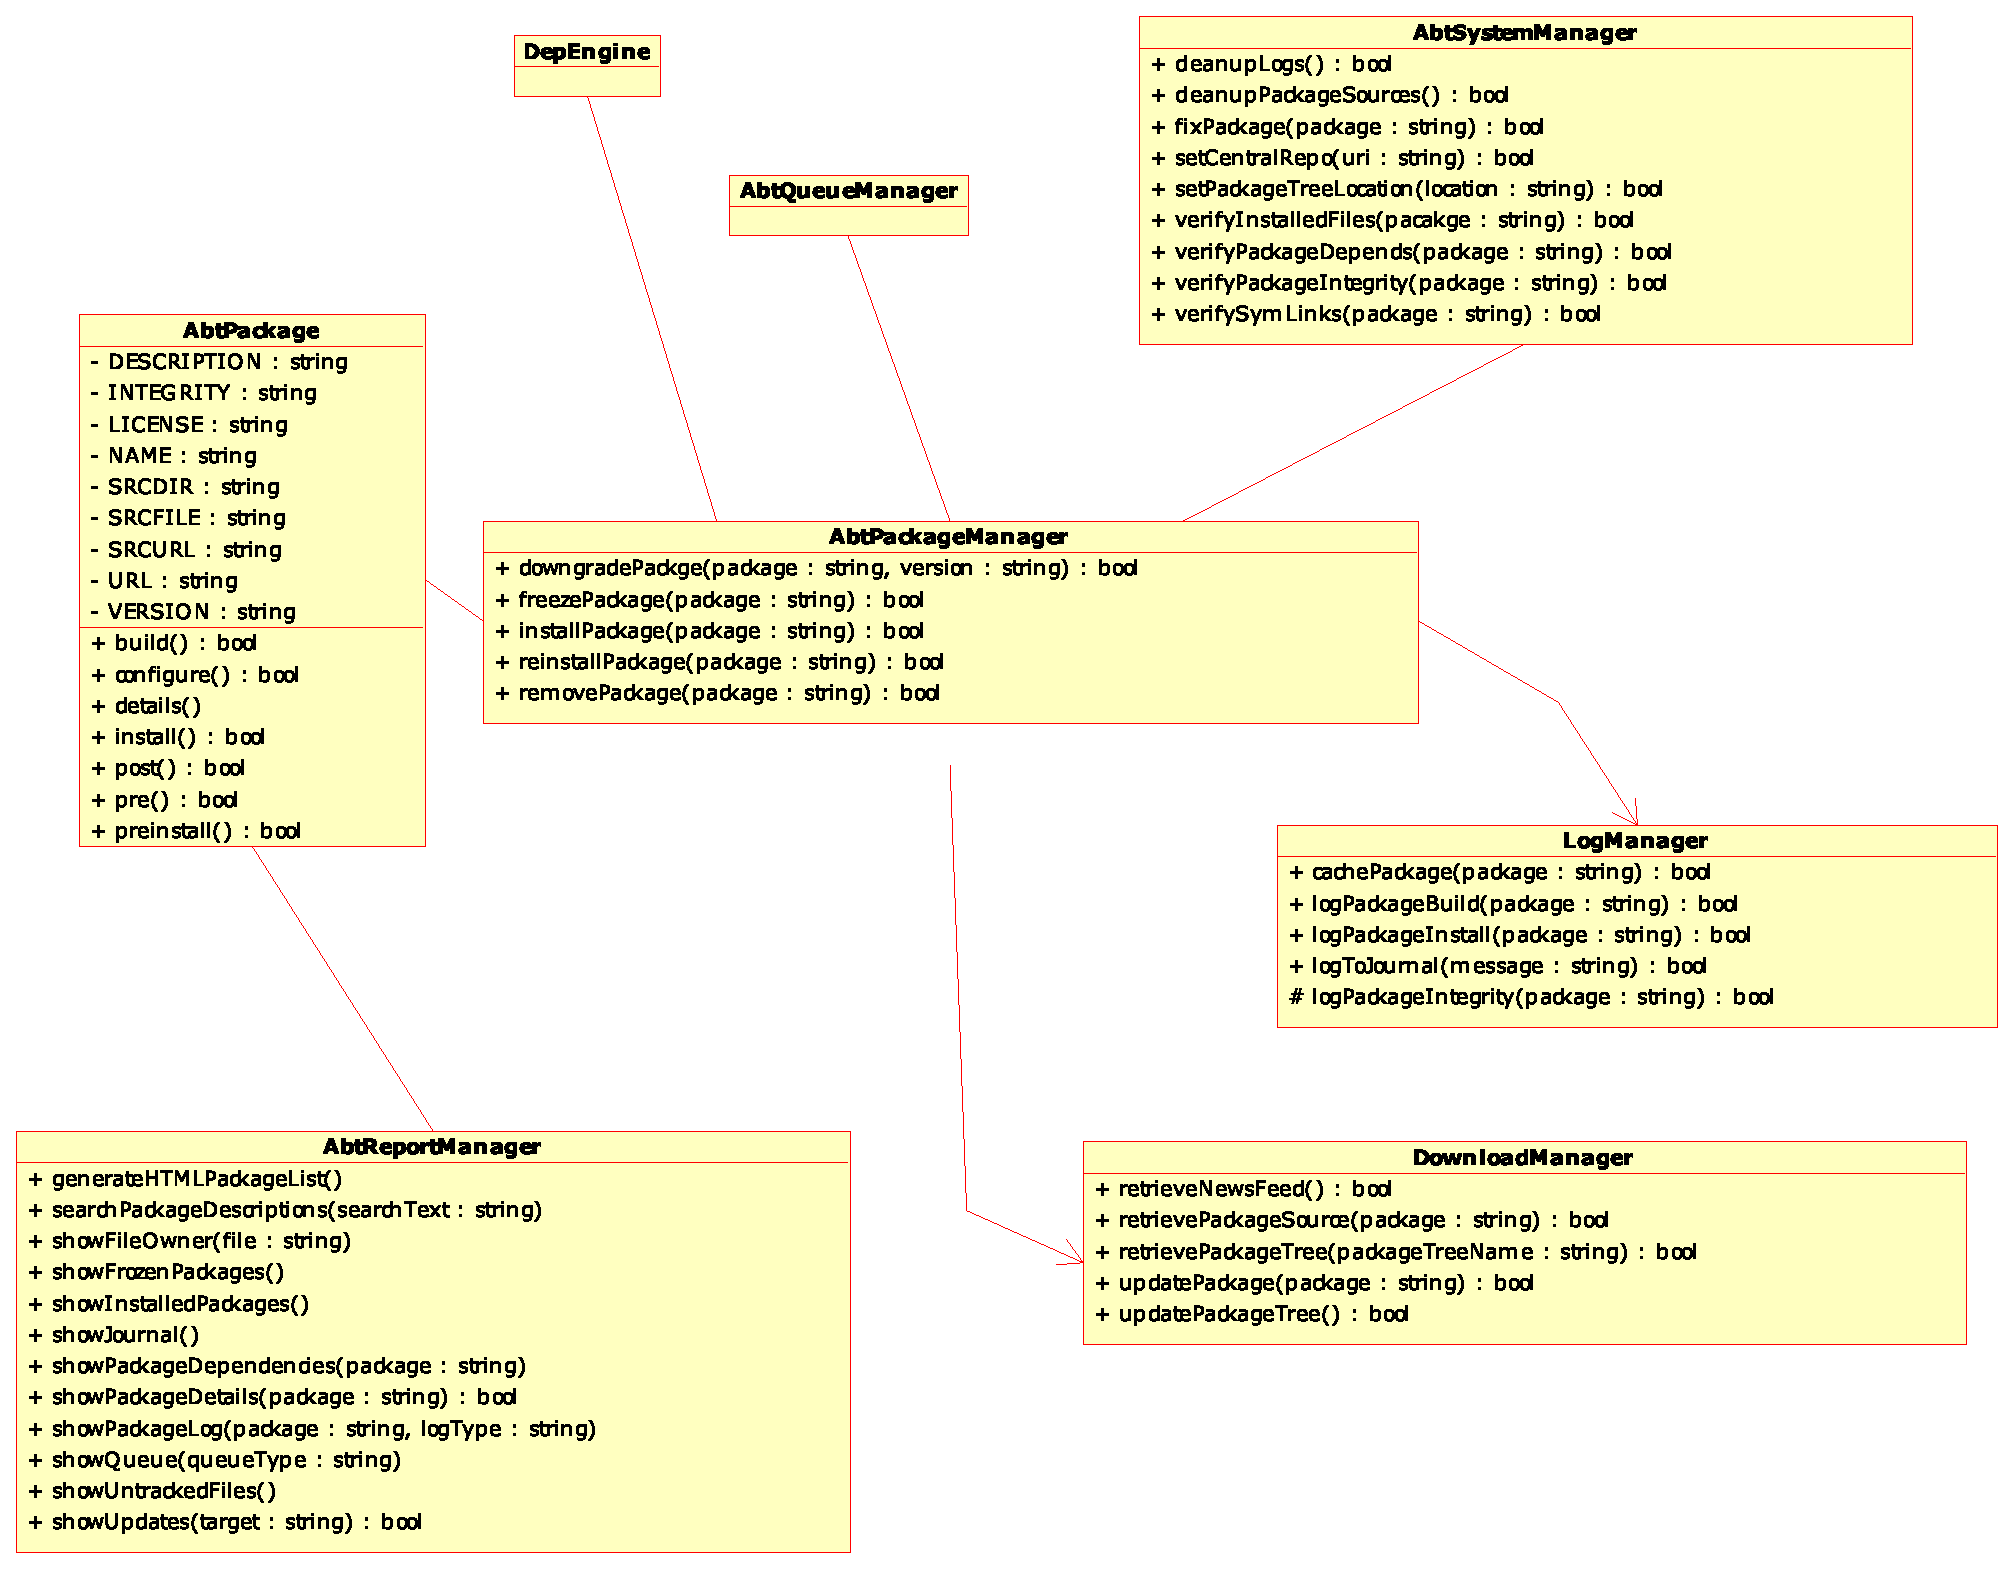
\includegraphics[width=16cm,height=22cm]{design/umlDesign.eps}
	\caption{The abt package manager UML class diagram}
	\label{fig:abtapi}
\end{figure}


\subsubsection{Repository names}
Providing the following repositories as subversion tags:

\begin{enumerate}
  \item \textbf{HEAD} - the current working repository.
  \item \textbf{TAGGED-RELEASE} - released version tagged with a unique name.
\end{enumerate}

\subsubsection{File storage}
The various files that are generated and needed by the abt package manager will be stored in the following locations:

\begin{itemize}
  \item package sources - \url{/var/spool/abt/}
  \item install info - \url{/var/state/abt/install/PKG_NAME/}
  \item cached info - \url{/var/state/abt/cached/PKG_NAME/}
  \item frozen info - \url{/var/log/abt/frozen.log}
  \item installed log - \url{/var/log/abt/installed.log}
  \item journal - \url{/var/log/abt/abt.log}
  \item newfeed - \url{/var/log/abt/news.log}
  \item install queue - \url{/var/log/abt/install.queue}
  \item tracking info - \url{/etc/abt/tracking.cfg}
\end{itemize}
